\sect{5. C\'omo jugar}

\begin{figure}[H]
\centering
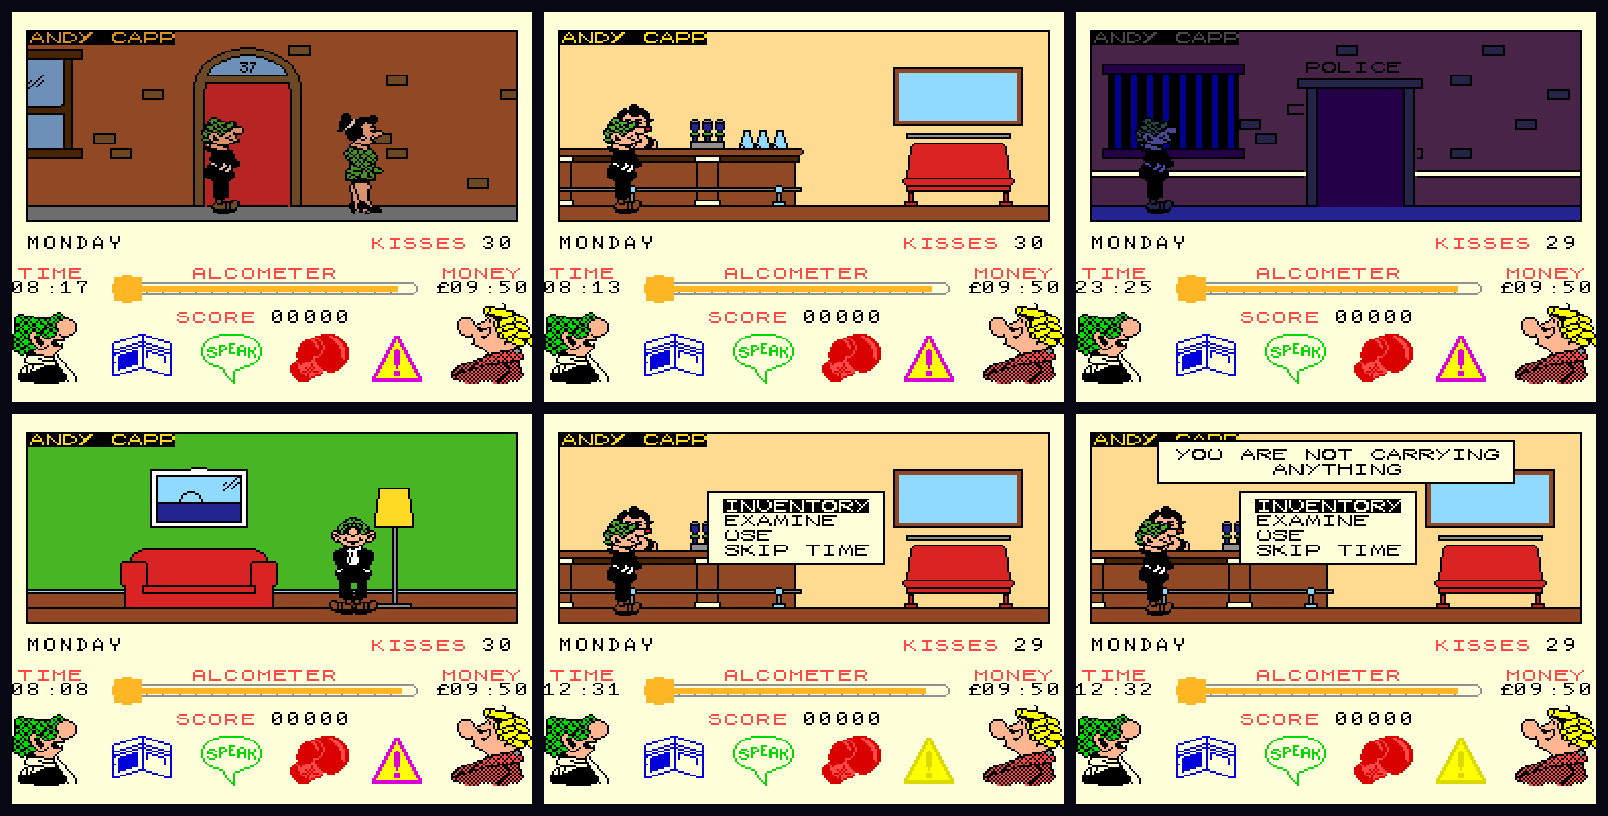
\includegraphics[width=\textwidth]{img/montage.png}
\caption{La calle de Andy, el bar, la comisar\'ia de noche, el sal\'on, el men\'u ACTION y un mensaje.}
\end{figure}

\textit{Es lunes por la ma\~nana y Andy anda de cabeza. Flo le reclama el cheque del paro y, si no lo consigue pronto, se ir\'a a casa de su madre. \textquestiondown Y qui\'en fregar\'a los platos entonces? Andy necesitar\'a toda su picard\'ia del norte para sacar dinero: sableando a los amigos, probando suerte en las carreras\ldots\ y sin cruzarse con el cobrador del alquiler ni con el polic\'ia, que van detr\'as de \'el.} (de las instrucciones originales)

\textbf{El objetivo} es conseguir \textbf{el giro} (el cheque del paro) y d\'arselo a Flo: con el giro en el bolsillo, ponte junto a ella y usa el giro (ACTION, USE). Para llegar ah\'i hay que resolver una cadena de encargos por todo el barrio.

\subsection*{El barrio}
Andy camina a izquierda y derecha por las calles; al llegar al borde de la pantalla pasa a la siguiente. En las esquinas y en las puertas de los edificios, ponte de cara y pulsa arriba. Hay dos calles largas unidas por calles laterales, con la casa de Andy (n\'umero 37), dos pubs \textit{Sparkling Ales}, la comisar\'ia, el juzgado, el ayuntamiento, la oficina de empleo, el quiosco, la casa de apuestas y la f\'abrica de Fred.

Los edificios tienen \textbf{horario}: los pubs abren de 11:00 a 15:00 y de 17:00 a 23:00; las tiendas y oficinas, de lunes a s\'abado de 8:00 a 17:00, y cierran el domingo. De noche las calles se oscurecen.

\subsection*{La gente}
Por las calles se mueven \textbf{Flo}, otra \textbf{mujer} con coleta, el \textbf{cobrador del alquiler} y varios \textbf{polic\'ias}. En los edificios hay gente tras el mostrador: el camarero, el quiosquero, el empleado de la oficina de empleo, el sargento de polic\'ia, el juez\ldots

\begin{itemize}
\item Para hablar o pelear con alguien tienes que \textbf{estar toc\'andolo}, salvo con la gente tras un mostrador.
\item Quien camina no te hace caso: primero l\'anzale un \textbf{beso} (abajo). Se queda parado un rato, embobado, y entonces puedes hablarle. Los besos tambi\'en sirven para dejar plantado a un polic\'ia y escapar. Se gastan: mira el contador.
\end{itemize}

\subsection*{Los iconos}
Pulsa \key{ESPACIO} y elige uno de los cuatro iconos de la parte de abajo:

\begin{description}
\item[CARTERA (TRANSACT)] Comprar y pagar: un peri\'odico en el quiosco, una pinta en el pub, el alquiler en el ayuntamiento, una apuesta en la casa de apuestas, un adelanto en la f\'abrica\ldots{} Lo que se ofrece depende de d\'onde est\'es. Andy empieza con \pounds 9.50.
\item[HABLAR (SPEAK)] Conversaciones y preguntas: \texttt{HAVE YOU SEEN MY RENT BOOK}, \texttt{HELLO}, \texttt{HAVE YOU SEEN MY GIRO}. En algunos sitios hay preguntas propias (en la oficina de empleo, en la f\'abrica\ldots).
\item[PELEAR (FIGHT)] A veces una pelea es la \'unica salida. Ver la secci\'on~7.
\item[ACCI\'ON (ACTION)] \texttt{INVENTORY} (lo que llevas), \texttt{EXAMINE} (mirar un objeto), \texttt{USE} (usar un objeto: beber la pinta, dar algo a alguien) y \texttt{SKIP TIME} (adelanta el reloj 4 horas, a costa de un poco de alcohol).
\end{description}

Los objetos no est\'an tirados por el suelo: se compran, te los dan o los encuentras haciendo lo adecuado en el sitio adecuado.

\subsection*{El alcohol\'imetro}
La barra del alcohol\'imetro baja con el tiempo. \textbf{Si se vac\'ia, se acaba la partida.} Se rellena con una \textbf{pinta}: c\'omprala en el pub con la cartera y b\'ebetela \textbf{dentro del pub} (ACTION, USE). Si sales a la calle con la pinta en la mano, la polic\'ia te busca. Cuando la barra est\'a llena, vuelves a tener 30 besos.

\subsection*{La polic\'ia, la c\'arcel y el juez}
Andy est\'a \textbf{en busca y captura} si se pelea o si sale del pub con la pinta. Mientras lo buscan, un polic\'ia que lo toque se lo lleva a pelear (a no ser que lo hayas dejado parado con un beso). Si pierdes una pelea, pasas la noche en el calabozo y a la ma\~nana siguiente el juez te pone una multa de \pounds 20: si no la pagas (o no puedes), se acaba la partida.

% ------------------------------------------------------------------
\sect{6. El marcador}

\begin{center}
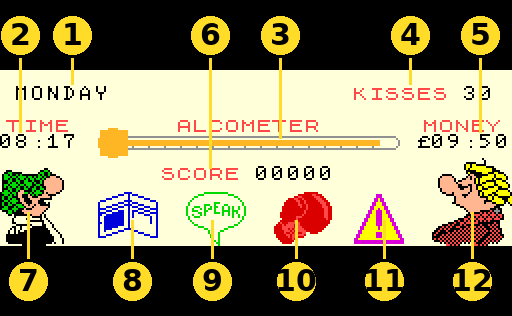
\includegraphics[width=0.9\textwidth]{img/hud.png}
\end{center}

\begin{tabularx}{\textwidth}{@{}clX@{}}
\toprule
\textbf{\tNo} & \textbf{\tElement} & \textbf{\tTellsYou}\\
\midrule
1 & D\'ia & El d\'ia de la semana. Cambia a medianoche.\\
2 & TIME & La hora (de 00:00 a 23:59). Un minuto de juego dura un segundo y medio.\\
3 & ALCOMETER & El alcohol que le queda a Andy. Si se vac\'ia, fin de la partida.\\
4 & KISSES & Los besos que te quedan.\\
5 & MONEY & El dinero, en libras y peniques.\\
6 & SCORE & La puntuaci\'on: se gana peleando.\\
7 & Andy & Andy Capp.\\
8 & Cartera & Icono TRANSACT: comprar y pagar.\\
9 & SPEAK & Icono para hablar.\\
10 & Guante & Icono para pelear.\\
11 & Se\~nal & Icono ACTION: objetos y SKIP TIME. El icono elegido parpadea.\\
12 & Flo & Flo, que espera su dinero.\\
\bottomrule
\end{tabularx}

% ------------------------------------------------------------------
\sect{7. Puntuaci\'on y final}

\begin{itemize}
\item La \textbf{puntuaci\'on} solo sube peleando: cada pu\~netazo que da Andy suma puntos, y ganar una pelea da una bonificaci\'on. La pelea se ve como una nube de polvo; la decide la suerte, golpe a golpe. Cada golpe que recibes baja el alcohol\'imetro, cada uno que das lo sube un poco.
\item \textbf{Ganas} cuando le das a Flo el giro: aparece \texttt{YOU HAVE WON}.
\item \textbf{Pierdes} si el alcohol\'imetro se vac\'ia, o si el juez te multa y no pagas.
\item No hay l\'imite de d\'ias: la semana sigue hasta que ganes o pierdas.
\end{itemize}

% ------------------------------------------------------------------
\sect{8. Consejos}

\begin{itemize}
\item Mant\'en lleno el alcohol\'imetro: ya sabes d\'onde se consigue, pero solo en horario de apertura.
\item Ap\'artate del polic\'ia: est\'as en la lista de buscados.
\item Si te apetece apostar, recuerda que los soplos no solo vienen en la car\'atula: lee bien el peri\'odico de las carreras.
\item Y si las cosas se ponen feas, siempre puedes buscar trabajo.
\item Habla con todo el mundo (con un beso antes, si camina) y pregunta por el giro y por la libreta del alquiler.
\item A algunas personas se las ablanda con un detalle.
\item SKIP TIME es \'util para llegar a la hora de apertura, pero cuesta alcohol.
\end{itemize}

{\small Los cuatro primeros consejos son los de las instrucciones originales.}
